\documentclass{beamer}
\useoutertheme{split}
\useinnertheme{circles}
\usecolortheme{custom}
\setbeamertemplate{navigation symbols}{}
\graphicspath{{graphics/}}

\newcommand*\oldmacro{}%
\let\oldmacro\insertshorttitle%
\renewcommand*\insertshorttitle{%
	\oldmacro\hspace{3.6cm}%
	    \insertframenumber\,/\,\inserttotalframenumber}

\title{Cache for HLS}
\subtitle{A multi-process architecture}
\author{Brignone Giovanni}
\titlegraphic{
\includegraphics[width=.4\textwidth]{polito_logo.png}}
%\institute{Politecnico di Torino}
\date{June 7, 2021}

\AtBeginSection[] {
	\tableofcontents[
		currentsection,
		sectionstyle=show/shaded,
		subsectionstyle=show/show/hide
	]
}

\begin{document}
\begin{frame}
	\maketitle
\end{frame}

\section{Introduction}
\subsection{Motivation}
\begin{frame}{Motivation}
	\begin{itemize}
		\item \textbf{Problem}:\\
			big arrays are mapped to \underline{DRAM} $\Rightarrow$
			performance \underline{bottlenecks}
		\item \textbf{Proposed solution}:\\
			cache module which should:
			\begin{itemize}
				\item store data to \underline{BRAMs}
				\item require \underline{minimal effort} to be
					integrated into any HLS design
			\end{itemize}
	\end{itemize}
\end{frame}

\section{Architecture}
\subsection{Inlined architecture}
\begin{frame}{Inlined architecture (Ma Liang)}
	\begin{minipage}{.7\textwidth}
		\begin{center}
			Array access $\rightarrow$ Inlined cache logic
		\end{center}

		\bigskip

		\begin{itemize}
			\item straightforward architecture
			\item cache logic mixed with application logic
			\item single-port only
		\end{itemize}
	\end{minipage}
	\begin{minipage}{.28\textwidth}
		\begin{center}
			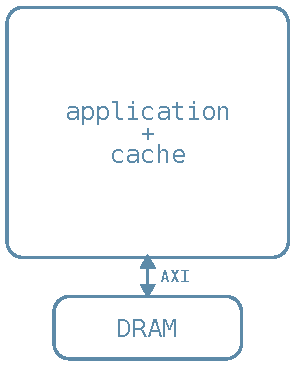
\includegraphics[width=.9\textwidth,height=.9\textheight,keepaspectratio]{liang_arch.pdf}
		\end{center}
	\end{minipage}
\end{frame}
\subsection{Multi-process architecture}
\begin{frame}{Multi-process architecture}
	\begin{minipage}{.7\textwidth}
		\begin{center}
			Array access $\rightarrow$ Request to separate module
		\end{center}
		\begin{itemize}
			\item decoupling between application and cache logic
				(communication through FIFOs)
			\item may support multiple ports (work in progress)
		\end{itemize}
	\end{minipage}
	\begin{minipage}{.28\textwidth}
		\begin{center}
			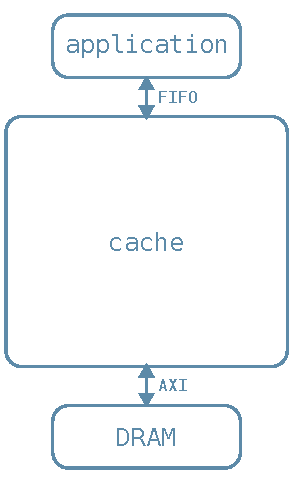
\includegraphics[width=.9\textwidth,height=.9\textheight,keepaspectratio]{complete_arch.pdf}
		\end{center}
	\end{minipage}
\end{frame}

\section{Implementation}
\subsection{Tools}
\begin{frame}{Tools}
	\texttt{C++} code compatible with \emph{Vitis HLS} (2020.2).
	\pause
	\begin{itemize}[<+->]
		\item \textbf{Multiple processes modeling}:\\
			infinite loops parallelized by:
			\begin{itemize}
				\item<.-> \underline{SW simulation:} \texttt{std::thread}
				\item<.-> \underline{Synthesis:} \texttt{DATAFLOW} with
					\textit{start propagation} disabled
			\end{itemize}
		\item \textbf{Inter-process communication}: \texttt{hls::stream} FIFOs
		\item \textbf{Performance optimization}:
			\begin{itemize}
				\item<.-> loop pipelining: new request each cycle
				\item<.-> automatic port widening: access one line at a time in DRAM
			\end{itemize}
		\item \textbf{Customization:} cache characteristics set through
			\texttt{template}
		\item \textbf{Limitations}: cannot override ``\texttt{[]~operator}''
			for \texttt{set} due to automatic \texttt{class} disaggregation
	\end{itemize}
\end{frame}

\subsection{Internal architecture}
\begin{frame}{Internal architecture}
	\begin{minipage}{.7\textwidth}
		\begin{itemize}[<+->]
		\item \textbf{Problem}: persuade HLS to schedule response writing
			to FIFO in case of HIT early in the pipeline
		\item \textbf{Proposed solution}: split the cache into two processes:
			\begin{enumerate}[<.->]
				\item \texttt{core}:
					\begin{itemize}
						\item manage requests from \texttt{application}
						\item keep cache data structures up-to-date
					\end{itemize}
				\item \texttt{mem\_if}:
					\begin{itemize}
						\item manage DRAM accesses
					\end{itemize}
			\end{enumerate}
		$\Rightarrow$ synthesizer job is simplified:\\
		if HIT, request is managed in 1 cycle
	\end{itemize}
	\end{minipage}
	\onslide<1->
	\begin{minipage}{.28\textwidth}
		\begin{center}
			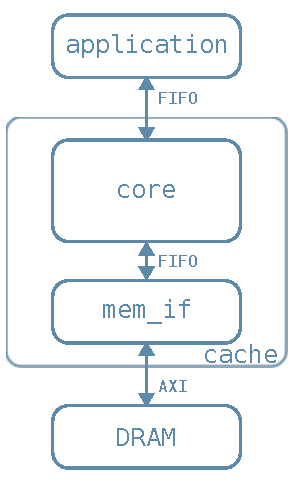
\includegraphics[width=.9\textwidth,height=.9\textheight,keepaspectratio]{internal_arch.pdf}
		\end{center}
	\end{minipage}
\end{frame}
\begin{frame}{\texttt{mem\_if} implementation}
	\framesubtitle{Functionality}
	\begin{minipage}{.7\textwidth}
		Manage DRAM accesses:
		\begin{enumerate}
			\item read request from \texttt{core}
			\item access DRAM
			\item write response to \texttt{core}
				(if \texttt{read} request)
		\end{enumerate}
	\end{minipage}
	\begin{minipage}{.28\textwidth}
		\begin{center}
			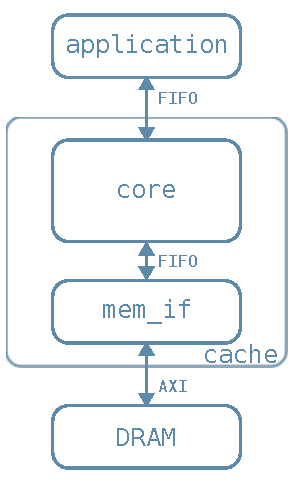
\includegraphics[width=.9\textwidth,height=.9\textheight,keepaspectratio]{internal_arch.pdf}
		\end{center}
	\end{minipage}
\end{frame}
\begin{frame}{\texttt{core} implementation}
	\framesubtitle{Functionality}
	\begin{minipage}{.7\textwidth}
		\begin{enumerate}[<+->]
			\item read request from \texttt{application}
			\item check if it is an HIT or a MISS
			\item if MISS: 
				\begin{itemize}
					\item if the cache line to be overwritten $\text{\texttt{line}}_{\text{old}}$
						has been modified, issue a \texttt{write}
						request of $\text{\texttt{line}}_{\text{old}}$ to \texttt{mem\_if}
					\item issue a \texttt{read} request of the
						requested line to \texttt{mem\_if}
					\item read \texttt{mem\_if} response and
						update BRAM

				\end{itemize}
			\item access BRAM
			\item write response to \texttt{application}
				(if \texttt{read})
		\end{enumerate}
	\end{minipage}
	\begin{minipage}{.28\textwidth}
		\begin{center}
			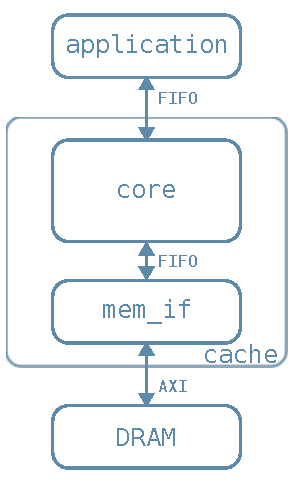
\includegraphics[width=.9\textwidth,height=.9\textheight,keepaspectratio]{internal_arch.pdf}
		\end{center}
	\end{minipage}
\end{frame}
\subsection{Problems and solutions}
\begin{frame}{BRAM dependencies~-~RAW \texttt{fill}}
	\framesubtitle{}
	\begin{minipage}{.7\textwidth}
		\begin{itemize}[<+->]
			\item \textbf{Problem}:
				reading BRAM immediately after it is written
				by the \texttt{fill} process causes an increase
				of II
			\item \textbf{Proposed solution}:
				store the \texttt{mem\_if} response in a buffer
				which can be immediately accessed and update BRAM
				afterwards
		\end{itemize}
	\end{minipage}
	\onslide<1->
	\begin{minipage}{.28\textwidth}
		\begin{center}
			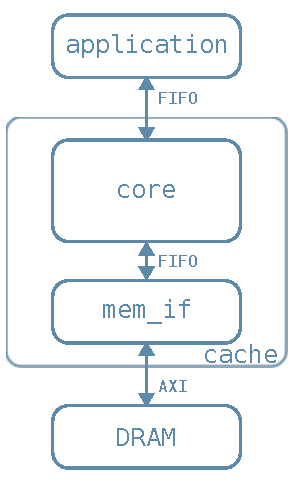
\includegraphics[width=.9\textwidth,height=.9\textheight,keepaspectratio]{internal_arch.pdf}
		\end{center}
	\end{minipage}
\end{frame}
\begin{frame}{BRAM dependencies~-~RAW \texttt{request}}
	\begin{minipage}{.7\textwidth}
		\begin{itemize}[<+->]
			\item \textbf{Problem}:
				reading BRAM immediately after it is written by
				a previous \texttt{write} request causes an
				increase of II
			\item \textbf{Proposed solution}:
				\texttt{raw\_cache} inside \texttt{cache}:
				\begin{itemize}[<.->]
					\item \texttt{write} request: store the
						written line to a buffer
					\item subsequent \texttt{read} request to
						the same line: access the buffer
						instead of BRAM
				\end{itemize}
		\end{itemize}
	\end{minipage}
	\onslide<1->
	\begin{minipage}{.28\textwidth}
		\begin{center}
			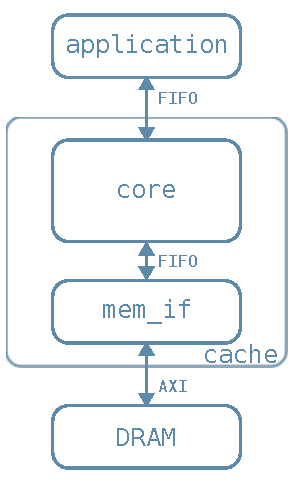
\includegraphics[width=.9\textwidth,height=.9\textheight,keepaspectratio]{internal_arch.pdf}
		\end{center}
	\end{minipage}
\end{frame}
\begin{frame}{Request optimization}
	\begin{minipage}{.7\textwidth}
		\begin{itemize}[<+->]
			\item \textbf{Problem}:
				\begin{itemize}[<.->]
					\item each FIFO access costs 1 cycle
					\item accesses to arrays are often sequential
				\end{itemize}
			\item \textbf{Proposed solution}:
				\texttt{l1\_cache} in the interface (\texttt{application}
				side):
				\begin{itemize}[<.->]
					\item \texttt{read} request:
						get the whole cache line, store it
						in a buffer and return the requested element
					\item subsequent \texttt{read} request to the same
						line: access the buffer
				\end{itemize}
			$\Rightarrow$ avoid passing through FIFOs
		\end{itemize}
	\end{minipage}
	\onslide<1->
	\begin{minipage}{.28\textwidth}
		\begin{center}
			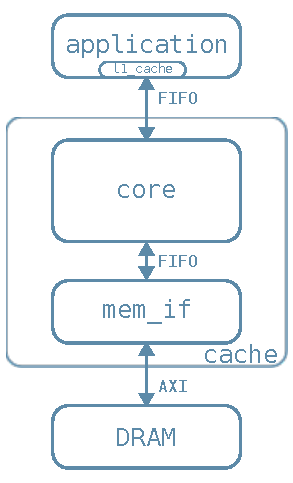
\includegraphics[width=.9\textwidth,height=.9\textheight,keepaspectratio]{l1_arch.pdf}
		\end{center}
	\end{minipage}
\end{frame}
\section{Results}
\subsection{Performance}
\begin{frame}{Performance}
	\begin{itemize}
		\item \textbf{Loop pipelining}:\\ both \texttt{core} and
			\texttt{mem\_if} loops pipelined with \texttt{II=1}
		\item \textbf{L1 HIT}: latency of 1 cycle
		\item \textbf{HIT}: latency of 6 cycles
	\end{itemize}
\end{frame}
\section{Future work}
\subsection{Multi-port cache}
\begin{frame}{Multi-port cache}
	\begin{itemize}[<+->]
		\item \textbf{Problem}: cache manages one request per cycle
			$\Rightarrow$ unrolling a loop which uses the cache is not
			trivial
		\item \textbf{Possible workarounds}:
			get multiple data elements for each request and do all
			the unroll in \texttt{application}; two possible ways:
			\begin{itemize}[<.->]
				\item \texttt{get\_line}: return a whole cache
					line
				\item pack multiple data elements in a single
					cache element (e.g. \texttt{hls::vector})
			\end{itemize}
		\item \textbf{Proposed solution}: provide $N$ ports, where $N$ is
			the unroll factor
	\end{itemize}
\end{frame}
\begin{frame}{Multi-port cache}
	\framesubtitle{Implementation}
	\begin{minipage}{.7\textwidth}
		\begin{itemize}[<+->]
			\item \textbf{Straightforward implementation}:
				\begin{itemize}[<.->]
					\item provide $N$ FIFOs on the interface
					\item unroll \texttt{core} loop by a factor $N$
				\end{itemize}
			\item \textbf{Problem}: all the $N$ requests may refer to the same line
				$\rightarrow$ each iteration must wait completion of
				previous one
		\end{itemize}
	\end{minipage}
	\onslide<1->
	\begin{minipage}{.28\textwidth}
		\begin{center}
			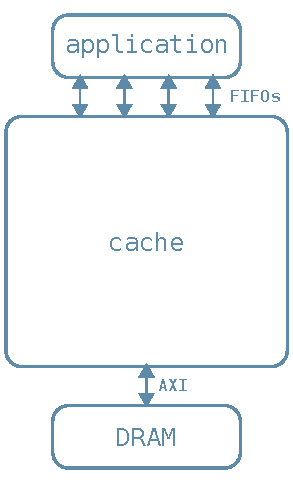
\includegraphics[width=.9\textwidth,height=.9\textheight,keepaspectratio]{multiport_arch.pdf}
		\end{center}
	\end{minipage}
\end{frame}
\begin{frame}{Multi-port cache}
	\framesubtitle{Implementation}
	\begin{minipage}{.7\textwidth}
		\begin{itemize}[<+->]
			\item \textbf{Proposed solution}:
				\begin{enumerate}[<.->]
					\item read all the $N$ requests
					\item check if they are all HIT
					\item if at least one MISS issue all the requests
						to \texttt{mem\_if}
					\item access BRAM
					\item write all the responses
				\end{enumerate}
				\pause
				\begin{itemize}
					\item cache addressing mode converted to an
						associative one
					\item possibly implement \texttt{core}
						at RTL to have full control
						on scheduling
				\end{itemize}
		\end{itemize}
	\end{minipage}
	\onslide<1->
	\begin{minipage}{.28\textwidth}
		\begin{center}
			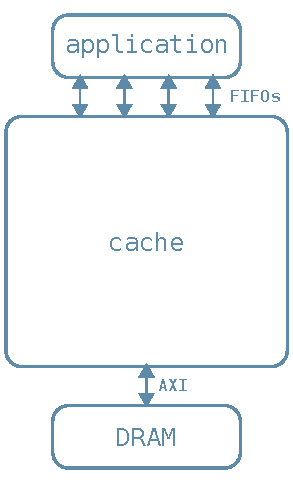
\includegraphics[width=.9\textwidth,height=.9\textheight,keepaspectratio]{multiport_arch.pdf}
		\end{center}
	\end{minipage}
\end{frame}

\end{document}

